\documentclass[sigconf]{acmart}

\settopmatter{printacmref=false} % Removes citation information below abstract
\renewcommand\footnotetextcopyrightpermission[1]{} % removes footnote with conference information in first column
\pagestyle{plain} % removes running headers

\usepackage[utf8]{inputenc}	
\usepackage[T1]{fontenc}

\usepackage{multirow}
\usepackage{booktabs} 
\usepackage{colortbl}
\usepackage{todonotes}
\usepackage{algorithm}
\usepackage{algorithmic}
\usepackage{pdfpages}
\usepackage{balance}
\usepackage{mdframed}
\usepackage{hyperref}

\usepackage[labelformat=simple]{subcaption}
\renewcommand\thesubfigure{(\alph{subfigure})}
\definecolor{Gray}{gray}{0.9}
 
\setcopyright{rightsretained}

\begin{document}
	
\title{Airbnb - New York’s Analysis}

\author{Jackson A. Prado Lima}
\affiliation{
	\institution{Department of Computer Science, Federal University of Paran\'{a}}
	\city{ CP:19081, CEP: 81531-980, Curitiba} 
	\state{Paran\'{a}}
	\country{Brazil}
}
\email{japlima@inf.ufpr.br} 
	
\renewcommand{\shortauthors}{J. A. Prado Lima}
\renewcommand{\shorttitle}{Airbnb - New York’s Analysis}

\begin{abstract}
	Airbnb is an outstanding hosting service used worldwide and provides information to its users in a simple and efficient manner, although this information is limited only to listings of its products. In this work, an analysis is made taking into account if incidents and cultural organizations influence the prices practiced in Airbnb. Besides, the prediction of new prices is carried out that the user can come to inform taking into account information of the current listings. The price forecast has some advantages when advising the user: on the price practiced (is too large or small), the mode of advertisement, or even on the investment decisions of the market analysis. To help in this task, the present work performs an analysis using graphs, maps and different types of machine learning.
\end{abstract}

%\keywords{BigData, Machine Learning, Airbnb} 

\maketitle

%%%%%%%%%%%%%%%%%%%%%%%%%%%%%%%%%%%%%%%%%%%%%%%%%%%%%%%%%%%%%%%%%%%%%%%%%%%%%%%%%%%%%%%%%%%%%%%%%%%%%%%%%%%%%%%%%%%%%%%%%%%
\vspace{-0.5cm}
\section{Introduction}

Airbnb was founded in August of 2008 and based in San Francisco, California. Airbnb is an online marketplace and hospitality service, enabling people to lease or rent short-term lodging including vacation rentals, apartment rentals, homestays, hostel beds, or hotel rooms. 

The company does not own any lodging; it is merely a broker and receives percentage service fees (commissions) from both guests and hosts in conjunction with every booking. It has over 3,000,000 lodging listings in 65,000 cities and 191 countries, and the host sets the cost of accommodation. Like all hospitality services, Airbnb is a form of collaborative consumption and sharing. Airbnb has two million rooms available - nearly three times more than that of the largest hotel chain in the world. 

How can we predict if a guest will continue booking rooms through Airbnb, and how can we predict if a host will continue listing out their property on Airbnb? Unlike traditional hotels, Airbnb relies on one group of its customers (hosts) to generate the supply of rooms for its guests. Thus, predicting customer loyalty, both on the host side and guest side, is arguably more important to Airbnb than to traditional hotels. In this paper, we try and capture this loyalty to Airbnb.

The data reveals that guests who stay with highly rated hosts are far more likely to return to Airbnb. For hosts, the best predictors of whether or not they will
continue to list through Airbnb is the recency and frequency of their listing.

%A proposta deste trabalho é utilizar três fontes de dados distintas na ferramenta de processamento de dados distribuídos Apache Spark e em seguida executar um algoritmo de aprendizado de máquina para aprender algo a partir dos dados que estão sendo utilizados.

%Para cumprir com as exigências do trabalho, foram selecionadas três bases de dados do governo brasileiro relativo às obras do PAC. O PAC, acrônimo de Programa de Aceleração do Crescimento, foi proposto pelo governo brasileiro em 2007 como um plano estratégico de resgate do planejamento e de retomada dos investimentos em setores estruturantes do país.

%O PAC possibilitou obras em diversos setores como saúde, educação, economia, turismo entre outras. Como o PAC abrange uma quantidade bastante grande de setores de investimento, há diversas possibilidades de pesquisa. Portanto foi escolhido um subconjunto dos dados para que os resultados fossem mais precisos. Desta forma, foi escolhido um setor de investimento, no caso o turismo. Esta escolha teve como base os dois grandes eventos esportivo de 2014 e 2016 (Copa do mundo de futebol e Olimpíadas respectivamente) e as bases de dados coletadas são de 2015, pareceu interessante investigar as obras do PAC que possuem cunho turístico.

%A seguir, na Seção \ref{Seção:Dados Utilizados}, será discutido um pouco mais sobre as bases de dados, os formatos disponíveis e o processamento realizado para possibilitar a utilização de aprendizado de máquina. Na Seção \ref{Seção:Investigando a base de dados} serão expostos e discutidos alguns resultados obtidos após a análise feita na base de dados utilizando apenas o Apache Spark, sem o uso de aprendizado de máquina. Esta análise tem como objetivo entender um pouco mais sobre os dados que foram utilizados neste trabalho. Em seguida, na Seção \ref{Seção:Predizendo dados} será proposta uma pergunta de pesquisa para ser respondida com o uso de aprendizagem de máquina, o experimento será explicado e os resultados expostos e discutidos. Já encaminhando para o fim do trabalho, na Seção \ref{Seção:Problemas encontrados} serão apresentados os problemas encontrados durante a execução deste trabalho. Por fim, na Seção \ref{Seção:Conclusão} serão relatadas as conclusões obtidas com este trabalho, em conjunto com os possíveis trabalhos futuros.

The paper is organized as follows. Section~\ref{sec:experiment_description} describes how the experimental evaluation was conducted. Section~\ref{sec:results} presents and analyses the results obtained. Finally, Section~\ref{sec:conclusion} concludes the paper and discusses the future work.

\vspace{-0.2cm}
\section{Experiment Description}
\label{sec:experiment_description}

The hypothesis of this work is that our approach is capable to recommend a local (district/borough) or a price to a user. To evaluate this, we consider uses maps, charts and machine learning.

According to our goals the experiment was guided by the following research question: \textbf{RQ:} ``How the incidents and cultural organizations impact on listing price?''.

To answer the RQ we conducted the evaluation in three phases: (i) Charts; (ii) Maps; and (iii) Machine Learning. In the first phase, we analyses the data distribution. In the second phase, we understand the impact of different factors using maps. In the last phase, we applies machine learning to predict some data.
	
From the main question we divided in other questions to understand different points:

\begin{itemize}
	\item \textbf{RQ1}: How the the cultural organizations impact on listing price?
	\item \textbf{RQ2}: How the the incidents impact on listing price?
	\item \textbf{RQ3}: How can we use average value rating, average location rating, etc. in the data?	
\end{itemize}

\vspace{-0.2cm}
\subsection{Target Data}
\label{sec:experiment_description:target_data}

The investigation focused on four dataset collected in open data sites. These dataset are as follows: 1) Listings, a dataset that is a Airbnb snapshot of 02 April, 2017; 2) Incidents, contains all incidents from New York for the year 2016; 3) Cultural Organizations, contains all cultural organizations from New York in 2017; and 4) NYC Borough, contains informations about boundaries of boroughs (districts). Further information about these datasets are available in the Table~\ref{tab:datasets}.

\begin{table*}[!htpb]
	\fontsize{9pt}{9pt}\selectfont
	\centering
	\caption{Characteristics of the data sets used in the experiment.}
	\label{tab:datasets}
	\begin{tabular}{ccp{10cm}cc}
		\toprule
		\textbf{\#} &              \textbf{Dataset}               & \textbf{Description}                                                                                                                          & \textbf{Size} & \textbf{Download} \\ \midrule
		     1      &         Listings~\cite{base:airbnb}         & Detailed listings data, including various attributes (features) of each listing such as number of bedrooms, bathrooms, location, etc.         &    153,7MB    &        csv        \\ \midrule
		     2      &       Incidents~\cite{base:incidents}       & All valid felony, misdemeanor, and violation crimes reported to the New York City Police Department (NYPD) for all complete quarters in 2016. &    124,2MB    &        csv        \\ \midrule
		     3      & Cultural Organizations~\cite{base:cultural} & Listing of all Cultural Organizations in the Department of Cultural Affairs directory.                                                        &    333,3kB    &        csv        \\ \midrule
		     4      &       NYC Borough~\cite{base:borough}       & Polygon boundaries of boroughs (water areas excluded).                                                                                        &    400,5kB    &      GeoJson      \\ \bottomrule
	\end{tabular}
\end{table*}

\vspace{-0.2cm}
\subsection{Settings}

In this step was used three different approaches to read the data (csv files): (i) SqlContext with databricks; (ii) parquet; and (iii) pandas. After, it was create a unique dataframe with the necessary informations. To help in the analsys, the Cultural Organizations and Incidents dataset received a score a they are like a column unique in the new dataframe. How we have 5 districts in New York, and to be easy, the Cultural Organizations and Incidents dataset were grouped and ranked in relation to the order (1-5), where 1 is the work and 5 the best. In this case, the datasets were ordered by the number in each district, ascendant for cultural organizations and descendant for the incidents. In the end, we have a unique dataset with 37043 rows.

\section{Results and Analysis}
\label{sec:results}

\begin{figure}[!htpb]
	\centering
	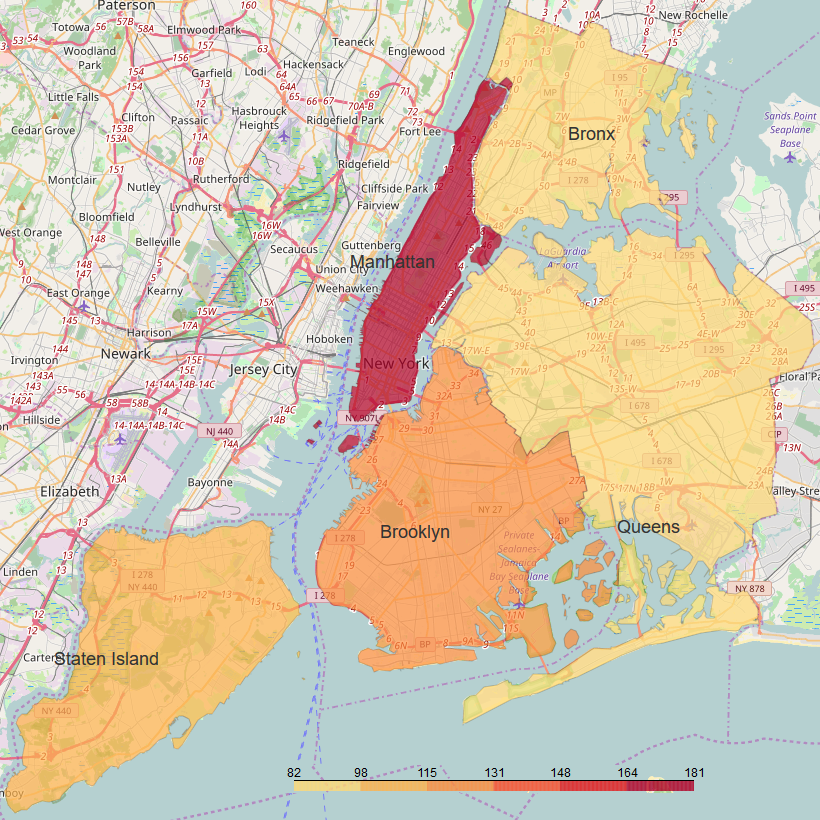
\includegraphics[width=\linewidth]{images/price_per_district}
	\caption{Mean Price per District}
	\label{fig:casPf}
\end{figure}

\begin{figure}[!htpb]
	\centering
	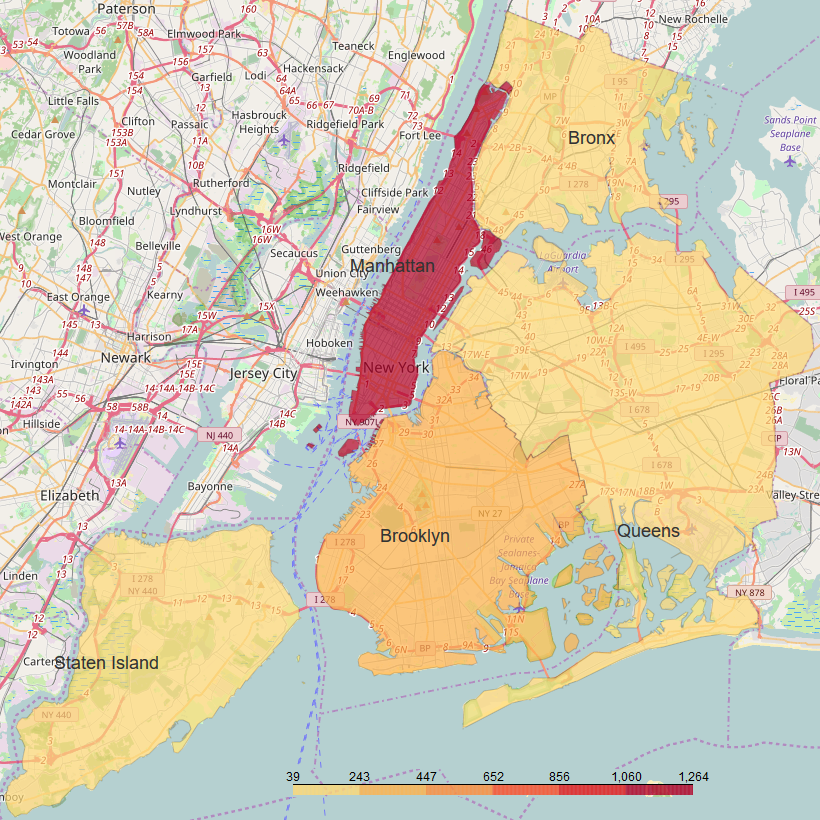
\includegraphics[width=\linewidth]{images/cultural_organizations_per_district}
	\caption{Number of Cultural Organizations per District}
	\label{fig:eshopPf}
\end{figure}

\begin{figure}[!htpb]
	\centering
	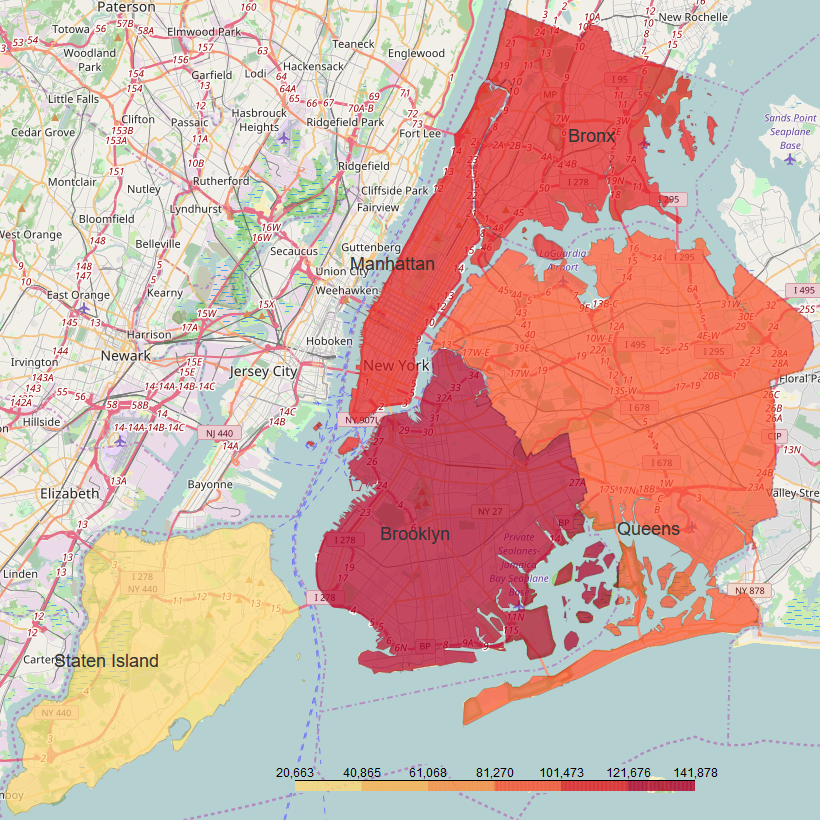
\includegraphics[width=\linewidth]{images/incidents_per_district}
	\caption{Number of Incidents per District}
	\label{fig:jamesPf}
\end{figure}

\begin{figure}[!htpb]
	\centering
	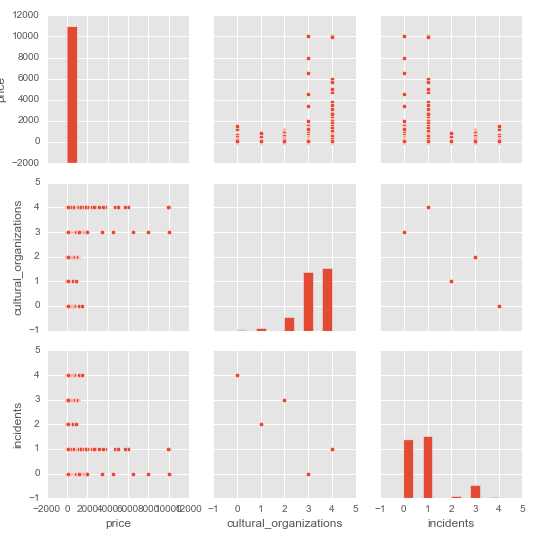
\includegraphics[width=\linewidth]{images/pairwise_relations_principal_features}
	\caption{}
	\label{fig:pairwiserelationsprincipalfeatures}
\end{figure}

\subsection{RQ1 - Comparing}

\subsection{RQ2 - UCB}

\subsection{Threats To Validity}
\label{sec:results:threats}

\section{Concluding Remarks}
\label{sec:conclusion}

\balance
\bibliographystyle{ACM-Reference-Format}
\bibliography{references} 

\end{document}